\chapter{Analysis}

\section{Actors}

\begin{itemize}
    \item \textbf{Unregistered User}: A visitor who has not logged in on the platform.
    
    \item \textbf{Registered User}: A user who has created an account on the platform.
    
    \item \textbf{Manager}: A registered user with administrative privileges.
\end{itemize}

\section{Functional Requirements}

The system should provide the following features for each type of user:

\begin{itemize}
    \item \textbf{Browse Media Contents}.
    
    \item \textbf{Search and Filter Media Contents}:
    \begin{itemize}
        \item Find specific manga or anime by title.
        \item Utilize basic filtering options to refine the media content list.
    \end{itemize}
    
    \item \textbf{View Media Content Trends}.
    
    \item \textbf{View Media Content}:
    \begin{itemize}
        \item View limited information about each media content.
    \end{itemize} 
    
    \item \textbf{View Media Content Details}:
    \begin{itemize}
        \item View detailed information about each media content.
        \item View reviews and ratings for each media content.
        \item View number of likes for each media content.
    \end{itemize}
    
    \item \textbf{Browse Users}.
    
    \item \textbf{Search Users by Username}.
    
    \item \textbf{View User}:
    \begin{itemize}
        \item View limited information about each user.
    \end{itemize} 
    
    \item \textbf{View User Details}:
    \begin{itemize}
        \item View detailed information about each user.
        \item View anime and manga liked by the user.
        \item View followers and following of the user.
    \end{itemize}
\end{itemize}

\subsection*{Unregistered User}

\begin{itemize}
    \item \textbf{Register/Login}:
    \begin{itemize}
        \item Create a new account to access additional features.
        \item Use valid credentials (email and password) to log into the account.
    \end{itemize}
\end{itemize}

\subsection*{Registered User}

\begin{itemize}
    \item \textbf{Logout}.
    
    \item \textbf{Profile Management}:
    \begin{itemize}
        \item Edit and update personal information (e.g., profile picture, bio).
        \item Delete own profile.
    \end{itemize}
    
    \item \textbf{Like/Unlike Media Contents}.
    
    \item \textbf{Follow/Unfollow Users}.
    
    \item \textbf{Review Media Contents}:
    \begin{itemize}
        \item Add comment and rating to manga and anime.
        \item Edit/Delete own reviews.
    \end{itemize}
    
    \item \textbf{Advanced Recommendations}:
    \begin{itemize}
        \item Receive media content suggestions based on user interactions and personal information.
        \item Receive users suggestions based on user interactions.
    \end{itemize}
\end{itemize}

\subsection*{Manager}

\begin{itemize}
    \item \textbf{Logout}.
    
    \item \textbf{Analytics Dashboard}:
    \begin{itemize}
        \item View user analytics (distribution and app rating).
        \item View manga analytics (trends and average rating).
        \item View anime analytics (trends and average rating).
    \end{itemize}
    
    \item \textbf{Content Management}:
    \begin{itemize}
        \item Add new media content (manga and anime).
        \item Update/Remove existing media content.
    \end{itemize}
\end{itemize}

\section{Non Functional Requirements}

\subsection*{Performance}

\begin{itemize}
    \item \textbf{Response Time}: The system should have low latency, with pages loading within an acceptable timeframe.
    
    \item \textbf{Scalability}: The system should be able to handle an increasing number of users and data without significant degradation in performance.
    
    \item \textbf{Concurrency}: The application should support multiple users simultaneously without performance bottlenecks. For very high traffic scenarios, acceptable delays may be introduced.
    
    \item \textbf{Availability}: The system should be available 24/7, with minimal downtime for maintenance.
    
    \item \textbf{Replication}: The system should have data replication to ensure data availability and fault tolerance.
\end{itemize}

\subsection*{Security}

\begin{itemize}
    \item \textbf{Controlled User Operations}: Users should only be able to perform operations that they are authorized to do.
\end{itemize}

\subsection*{Data Integrity}

\begin{itemize}
    \item \textbf{Data Consistency}: The system should maintain data consistency across all components and databases.
\end{itemize}

\subsection*{User Interface}

\begin{itemize}
    \item \textbf{Responsiveness}: The user interface should be responsive, providing a consistent and seamless experience across various devices and screen sizes.
    
    \item \textbf{Intuitiveness}: The interface should be user-friendly, with clear navigation and easily understandable features.
\end{itemize}

\section{UML class diagram}

\begin{figure}[h]\label{uml class diagram}
    \centering
    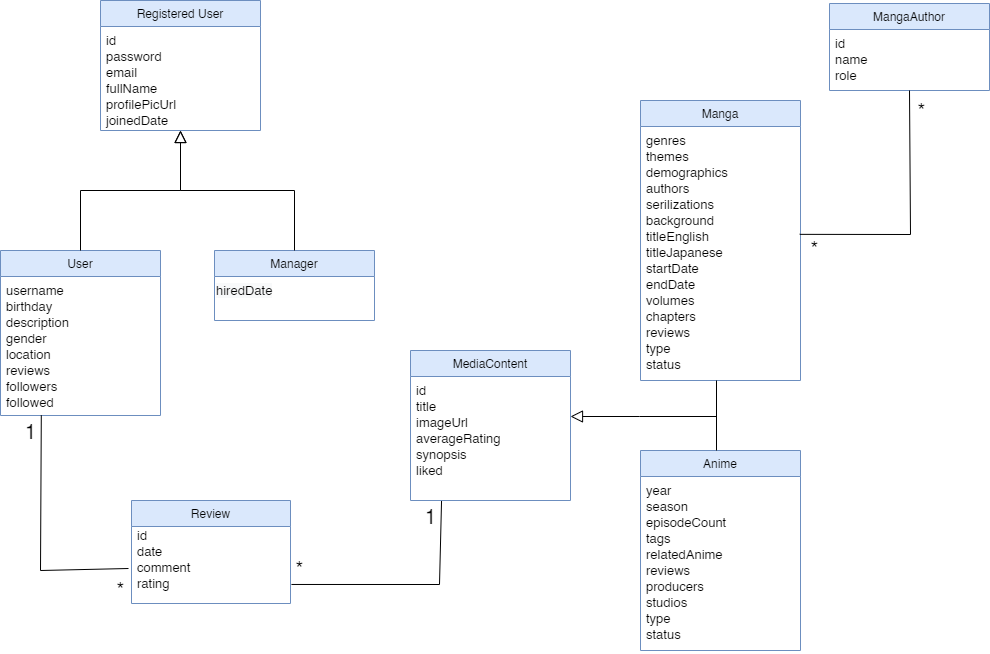
\includegraphics[width=\linewidth]{Media/Class Diagram.png}
\end{figure}

\newpage

\section{UML use case diagram}

\begin{figure}[h]\label{uml use case diagram}
    \centering
    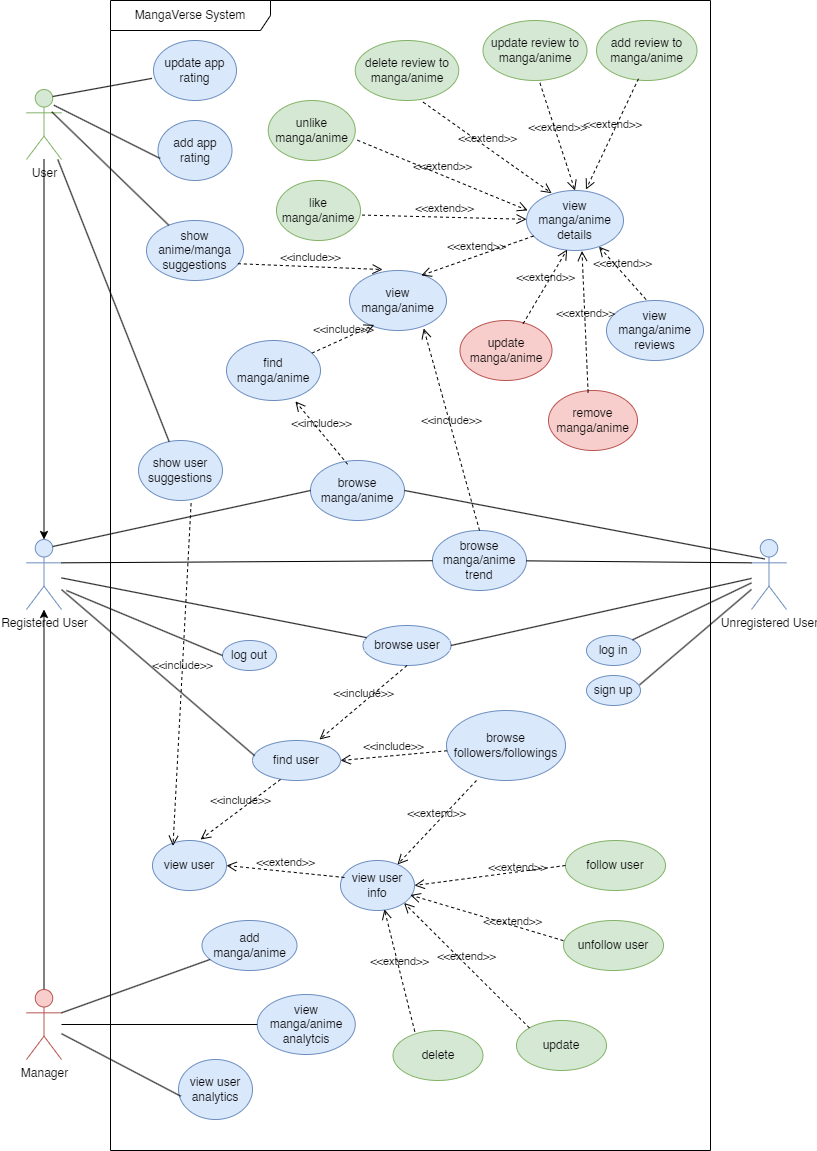
\includegraphics[width=0.85\textwidth]{Media/use_case.png}
\end{figure}

\newpage

\section{Scenarios}

\definecolor{lightblue}{rgb}{0.86, 0.92, 1.0}
\renewcommand{\arraystretch}{1.5}
\setlength{\arrayrulewidth}{1pt} % Adjusts the thickness of \hline

\begin{longtable}{|p{0.25\textwidth}|p{0.75\textwidth}|}
    \hline
    \rowcolor{lightblue}
    \textbf{Use Case} & \textbf{Register Account} \\
    \hline
    Primary Actor & Unregistered User\\
    \hline
    Description & Allows user to sign up\\
    \hline
    Pre-conditions & The account must not be already exist\\
    \hline
    Main Event Steps &   1. The user navigates to the registration page. \\
    & 2. The user fills out the registration form with valid information. \\
    & 3. The system validates the entered information. \\
    & 4. After successful validation, the system created a new user account \\
    \hline
    Post-conditions &The user is registered to the system \\
    \hline
    Correlated Use Cases & -\\
    \hline
\end{longtable}

\begin{longtable}{|p{0.25\textwidth}|p{0.75\textwidth}|}
    \hline
    \rowcolor{lightblue}
    \textbf{Use Case} & \textbf{Log In} \\
    \hline
    Primary Actor &Registered User\\
    \hline
    Description & Allows user to login \\
    \hline
    Pre-conditions & The user must not be already logged in\\
    \hline
    Main Event Steps & 1. The user navigates to the login page. \\
    & 2. The system shows the login form to the user and asks for email and password \\
    & 3. The user enters valid login credentials. \\
    & 4. The system validates the entered credentials \\
    & 5. After successful validation, the system logs the user. \\
    \hline
    Post-conditions & 1. The user is authenticated and logged in \\
    & 2. The user is redirected to the main page for registered user. \\
    \hline
    Correlated Use Cases & -\\
    \hline
\end{longtable}

\begin{longtable}{|p{0.25\textwidth}|p{0.75\textwidth}|}
    \hline
    \rowcolor{lightblue}
    \textbf{Use Case} & \textbf{Log Out} \\
    \hline
    Primary Actor &Registered User\\
    \hline
    Description & Allows user to logged out\\
    \hline
    Pre-conditions & The user must be logged in\\
    \hline
    Main Event Steps & The system starts the logout process \\
    \hline
    Post-conditions &The user is logged out. \\
    & The user is directed to the main page \\
    \hline
    Correlated Use Cases &-\\
    \hline
\end{longtable}

\newpage

\begin{longtable}{|p{0.25\textwidth}|p{0.75\textwidth}|}
    \hline
    \rowcolor{lightblue}
    \textbf{Use Case} & \textbf{Browse Anime/Manga} \\
    \hline
    Primary Actor & Registered User, Unregistered User\\
    \hline
    Description & Allows both registered and unregistered users to browse anime and manga\\
    \hline
    Pre-conditions & - \\
    \hline
    Main Event Steps & 1. The user navigates to the browse section. \\
    & 2. The system displays a list of available anime and manga. \\
    \hline
    Post-conditions & 1. The user will view the list of anime or manga\\
    & 2. The user can filter or sort the list based on various criteria. \\
    \hline
    Correlated Use Cases & Find Anime/Manga\\
    \hline
\end{longtable}

\begin{longtable}{|p{0.25\textwidth}|p{0.75\textwidth}|}
    \hline
    \rowcolor{lightblue}
    \textbf{Use Case} & \textbf{Find Anime/Manga} \\
    \hline
    Primary Actor & Registered User, Unregistered User\\
    \hline
    Description & Allows users to search for specific anime or manga. \\
    \hline
    Pre-conditions & - \\
    \hline
    Main Event Steps &  1. The user navigates to the search section of anime/manga. \\
    & 2. The user enters search criteria (e.g., title). \\
    & 3. The system retrieves a list of available anime/manga. \\
    & 4. The user can apply filters or sort the list. \\
    \hline
    Post-conditions & The system displays a result of the search \\
    & The user views a list of anime/manga matching with the used criteria\\
    \hline
    Correlated Use Cases &View Anime/Manga \\
    \hline
\end{longtable}

\begin{longtable}{|p{0.25\textwidth}|p{0.75\textwidth}|}
    \hline
    \rowcolor{lightblue}
    \textbf{Use Case} & \textbf{View Anime/Manga} \\
    \hline
    Primary Actor & Registered User, Unregistered User\\
    \hline
    Description &Allows users to view details of a specific anime or manga \\
    \hline
    Pre-conditions & -\\
    \hline
    Main Event Steps & 1. The user selects an anime or manga from the list or search results.\\
    & 2. The system displays pre information about the selected anime/manga. \\
    \hline
    Post-conditions & The user views pre information about the selected anime/manga\\
    \hline
    Correlated Use Cases & -\\
    \hline
\end{longtable}

\newpage

\begin{longtable}{|p{0.25\textwidth}|p{0.75\textwidth}|}
    \hline
    \rowcolor{lightblue}
    \textbf{Use Case} & \textbf{View Anime/Manga Details} \\
    \hline
    Primary Actor & Registered User, Unregistered User\\
    \hline
    Description & Allows users to view all the information about the specific anime or manga including reviews\\
    \hline
    Pre-conditions & -\\
    \hline
    Main Event Steps & 1. The user selects an anime or manga. \\
    & 2. The system retrieves detailed information, including reviews. \\
    \hline
    Post-conditions & \\
    \hline
    Correlated Use Cases & -\\
    \hline
\end{longtable}


\begin{longtable}{|p{0.25\textwidth}|p{0.75\textwidth}|}
    \hline
    \rowcolor{lightblue}
    \textbf{Use Case} & \textbf{View Anime/Manga Reviews} \\
    \hline
    Primary Actor & Registered User, Unregistered User\\
    \hline
    Description &Allows users to view reviews of a specific anime or manga\\
    \hline
    Pre-conditions & - \\
    \hline
    Main Event Steps & 1. The user navigates to the reviews section of a specific anime or manga.\\
    & 2. The system retrieves the reviews. \\
    & 3. The system displays the reviews to the user. \\
    \hline
    Post-conditions & The user views the reviews of the specific anime or manga\\
    \hline
    Correlated Use Cases & - \\
    \hline
\end{longtable}


\begin{longtable}{|p{0.25\textwidth}|p{0.75\textwidth}|}
    \hline
    \rowcolor{lightblue}
    \textbf{Use Case} & \textbf{Show Anime/Manga Suggestions} \\
    \hline
    Primary Actor &User \\
    \hline
    Description & Allows users to view anime or manga suggestions based on their likes or followings\\
    \hline
    Pre-conditions & User must be logged in\\
    \hline
    Main Event Steps & 1. The user navigates to the suggestions part of the main page. \\
    & 2. The system retrieves suggestions based on user preferences and followings. \\
    & 3. The system displays the suggestions to the user. \\
    \hline
    Post-conditions & The user views the suggested anime or manga\\
    \hline
    Correlated Use Cases & View Manga/Anime\\
    \hline
\end{longtable}

\newpage

\begin{longtable}{|p{0.25\textwidth}|p{0.75\textwidth}|}
    \hline
    \rowcolor{lightblue}
    \textbf{Use Case} & \textbf{Browse Anime/Manga Trend} \\
    \hline
    Primary Actor & Registered USer, Unregistered User\\
    \hline
    Description &Allows users to browse trending anime or manga\\
    \hline
    Pre-conditions & User must be logged in\\
    \hline
    Main Event Steps & 1. The user navigates to the trending section of the main page. \\
    & 2. The system retrieves trending anime or manga. \\
    & 3. The system displays the trending items to the user. \\
    \hline
    Post-conditions &-\\
    \hline
    Correlated Use Cases &View Anime/Manga \\
    \hline
\end{longtable}


\begin{longtable}{|p{0.25\textwidth}|p{0.75\textwidth}|}
    \hline
    \rowcolor{lightblue}
    \textbf{Use Case} & \textbf{Like Anime/Manga} \\
    \hline
    Primary Actor & User\\
    \hline
    Description &Allows users to like an anime or manga\\
    \hline
    Pre-conditions &User must be logged in \\
    \hline
    Main Event Steps & 1. The user clicks the like or unlike button. \\
    & 2. The system updates the like status. \\\\
    \hline
    Post-conditions &1. The anime or manga is liked or liked by the user and added to the liked anime/manga list\\
    &2. The appearance of like button is changed to filled version of the button\\
    \hline
    Correlated Use Cases &- \\
    \hline
\end{longtable}


\begin{longtable}{|p{0.25\textwidth}|p{0.75\textwidth}|}
    \hline
    \rowcolor{lightblue}
    \textbf{Use Case} & \textbf{Add Review to Anime/Manga} \\
    \hline
    Primary Actor & User\\
    \hline
    Description &Allows user to make comment or rating for specific anime/manga\\
    \hline
    Pre-conditions & User must be logged in\\
    \hline
    Main Event Steps &  1. The user selects an anime or manga. \\
    & 2. The user navigates to the review section. \\
    & 3. The user adds a review that can be either comment or rating the anime/manga\\
    & 4. The system ensures that at least one of the comment or rate value is filled\\
    & 5. The system saves the review and updates the latest reviews \\
    \hline
    Post-conditions & The review is added to the specific anime/manga and visible on the page\\
    \hline
    Correlated Use Cases & - \\
    \hline
\end{longtable}

\newpage

\begin{longtable}{|p{0.25\textwidth}|p{0.75\textwidth}|}
    \hline
    \rowcolor{lightblue}
    \textbf{Use Case} & \textbf{Show User Suggestions} \\
    \hline
    Primary Actor &User \\
    \hline
    Description &Allows users to view suggested users based on similar tastes or may know\\
    \hline
    Pre-conditions & User must be logged in\\
    \hline
    Main Event Steps &1. The user navigates to the profile page's suggested users section\\
    &2. The system retrieves suggested users based on user preferences and followings\\
    &3. The system displays the suggested users to the user\\
    \hline
    Post-conditions & The user views the suggested users.\\
    \hline
    Correlated Use Cases & View User\\
    \hline
\end{longtable}


\begin{longtable}{|p{0.25\textwidth}|p{0.75\textwidth}|}
    \hline
    \rowcolor{lightblue}
    \textbf{Use Case} & \textbf{Find User} \\
    \hline
    Primary Actor & Registered User, Unregistered User\\
    \hline
    Description & Allows users to search for specific users according to their usernames\\
    \hline
    Pre-conditions &- \\
    \hline
    Main Event Steps & 1. The user navigates to the user user search section of the page. \\
    & 2. The user enters search criteria. \\
    & 3. The system retrieves matching users based on criteria. \\
    & 4. The system displays the search results to the user. \\
    \hline
    Post-conditions & The user views the search results. \\
    \hline
    Correlated Use Cases & View User\\
    \hline
\end{longtable}

\begin{longtable}{|p{0.25\textwidth}|p{0.75\textwidth}|}
    \hline
    \rowcolor{lightblue}
    \textbf{Use Case} & \textbf{Browse Followings/Followers} \\
    \hline
    Primary Actor & Registered User, Unregistered User\\
    \hline
    Description & Allows users to browse their or others followers and followings\\
    \hline
    Pre-conditions & - \\
    \hline
    Main Event Steps & 1. The user navigates to the profile page.\\
    & 2. The user selects the followers or followings section. \\
    & 3. The system retrieves the list of followers or followings. \\
    & 4. The system displays the list to the user. \\
    \hline
    Post-conditions & The user views their followers and followings.\\
    \hline
    Correlated Use Cases &Find User,View User Info \\
    \hline
\end{longtable}

\newpage

\begin{longtable}{|p{0.25\textwidth}|p{0.75\textwidth}|}
    \hline
    \rowcolor{lightblue}
    \textbf{Use Case} & \textbf{Follow User} \\
    \hline
    Primary Actor & Registered User\\
    \hline
    Description & Allows users to follow another user\\
    \hline
    Pre-conditions & User must be logged in\\
    \hline
    Main Event Steps &  1. The user selects a user to follow \\
    & 2. The user navigates to that user's profile page. \\
    & 3. The systems displays the profile of other user. \\
    & 4. The user clicks the follow button. \\
    & 5. The system add the user to the following list of the other user and updates the count on the profile \\
    & 6. The system updates the follow/unfollow status. \\
    \hline
    Post-conditions &The user starts to follow the other user \\
    \hline
    Correlated Use Cases & -\\
    \hline
\end{longtable}


\begin{longtable}{|p{0.25\textwidth}|p{0.75\textwidth}|}
    \hline
    \rowcolor{lightblue}
    \textbf{Use Case} & \textbf{View User Information} \\
    \hline
    Primary Actor & Registered User, Unregistered User\\
    \hline
    Description & Allows users to view detailed information about another user\\
    \hline
    Pre-conditions & -\\
    \hline
    Main Event Steps& 1. The user selects a user from the list or search results or browse \\
    & 2. The system retrieves detailed information about the selected user. \\
    & 3. The system displays the detailed information to the user. \\
    \hline
    Post-conditions &The user views detailed information about the selected user.  \\
    \hline
    Correlated Use Cases & - \\
    \hline
\end{longtable}

\begin{longtable}{|p{0.25\textwidth}|p{0.75\textwidth}|}
    \hline
    \rowcolor{lightblue}
    \textbf{Use Case} & \textbf{View Analytics} \\
    \hline
    Primary Actor & Manager \\
    \hline
    Description & Allows managers to view analytics related to users and anime/manga\\
    \hline
    Pre-conditions & The user must be logged in with manager credentials\\
    \hline
    Main Event Steps & 1. The manager navigates to the analytics section of their page \\
    & 2. The system retrieves analytics data. \\
    & 3. The system displays the analytics data to the manager. \\
    \hline
    Post-conditions & The manager views the analytics data.\\
    \hline
    Correlated Use Cases & -\\
    \hline
\end{longtable}

\newpage

\section{Data Modeling}

\subsection{Data Collection}

\textit{Sources:}
\href{https://myanimelist.net/}{myAnimeList.net}, 
\href{https://anilist.co/}{anilist.co},
\href{https://kitsu.io/}{kitsu.io},
\href{https://livechart.me/}{livechart.me}, \\
\href{https://anime-planet.com/}{anime-planet.com},
\href{https://notify.moe/}{notify.moe},
\href{https://anisearch.com/}{anisearch.com},
\href{https://anidb.net/}{anidb.net}.

\vspace{\baselineskip}

\textit{Description:} The datasets contain information about anime, manga, users, and scores. 
Anime and reviews are stored in separate CSV files. The manga dataset is collected from myAnimeList.net, 
scraped using the \href{https://myanimelist.net/apiconfig/references/api/v2}{Official API} and \href{https://docs.api.jikan.moe/}{Jikan API}.

\vspace{\baselineskip}

\textit{Variety:} Anime are collected from 8 different sources, manga from one source, 
and users/reviews from the same sources (myAnimeList and Anime-Planet). 
The data is structured across 4 CSV files and a JSON file.

\vspace{\baselineskip}

\textit{Volume:} $\sim$3 GB\@. The datasets contain approximately 10 million reviews, 40k anime entries, 70k manga entries, 
and 200k users.

\subsection{Data Cleaning and Preprocessing}

The data cleaning and preprocessing involved several steps to ensure consistency and usability of the datasets:

\begin{itemize}
    \item \textbf{Data Integration and Reduction}: Integrating anime, reviews, and user data from various sources 
    required dealing with non-unique IDs across datasets. To ensure proper integration, 
    new unique IDs were generated for each entity. Due to issues with data quality, 
    a significant number of users and their associated reviews were removed. This process resulted in a 
    refined dataset containing 10,000 users and 600,000 reviews.
 
    \item \textbf{Review Comment Generation}: Some sources lacked explicit comments for reviews. To address this, 
    a script was employed to generate generic comments based on the review ratings, ensuring completeness of the review dataset.
    
    \item \textbf{Synthetic Data Generation}: Many users did not have sufficient reviews for meaningful analytics. 
    Synthetic reviews were generated to supplement these users, enabling more robust analysis 
    of user interactions and content preferences.
    
    \item \textbf{Data Pruning}: Extraneous information about users, anime, and manga that were 
    not relevant to the project goals were removed to streamline the datasets.
    
    \item \textbf{Data Augmentation}: Essential user information such as email, password, and profile picture, 
    which were necessary for user management features, were added to the dataset.
    
    \item \textbf{Consistency Checks}: Before insertion into the Document DB collections, rigorous data consistency checks were conducted to 
    uphold accuracy and reliability. For instance, chronological consistency was enforced for fields such as the joined date, 
    ensuring it fell after the user's birthdate and before any related review dates. Additionally, user locations were validated 
    to ensure they mapped to valid countries. Upon insertion, Document DB's ids were utilized for entity linking and to maintain data integrity.

    \item \textbf{Graph Database Population}: Fake relationships were created, such as follow relationships between users and like relationships 
    between users and anime/manga, to populate the graph database.
\end{itemize}

\vspace{\baselineskip}

These steps were crucial in preparing the datasets for effective utilization within the MangaVerse platform, 
ensuring data quality and integrity across all components.

\vspace{\baselineskip}

Python was predominantly used for data preprocessing tasks, leveraging its flexibility and extensive libraries. 
Additionally, Java was employed for specific tasks such as adding and updating redundancies in the document database.